% Drawing 69/01-12 -- folder 69, batch 01, archive page 13 (PDF page 14).
% Transcription: à gauche, un prisme vu d'en haut : triangle $u, v, w$ en bas, sommets $\alpha_4$, $\beta_4$, $\gamma_4$ au milieu (le triangle $\alpha_4 \gamma_4 \beta_4$ repassé), $\alpha'_4$, $\beta'_4$, $\gamma'_4$ à l'extérieur
% Kind: prism seen from above. Method 2 (schematic redraw from the facsimile). Status: ok.
% Notes: Nine vertices placed once, every edge drawn between them: the outer gamma'_4 (top), alpha'_4 (left), beta'_4 (right); the middle triangle alpha_4 gamma_4 beta_4, its sides alpha_4 gamma_4 and alpha_4 beta_4 inked over (thick), gamma_4 beta_4 thin; the lower triangle u, v with w above them (w u, w v, u v). Joining strokes as on the page: gamma'_4 alpha'_4, gamma'_4 beta'_4, gamma'_4 gamma_4 (thick), alpha'_4 gamma_4, gamma_4 beta'_4 (thick), alpha'_4 u (doubled on the page, drawn once), beta_4 v, gamma_4 w (faint), and a broken stroke from beta'_4 towards v (drawn faint, short of v as on the page). Which strokes join the levels is a reading of overlapping lines. Redrawn 2026-11-09 (issue 128): vertices placed once and every edge drawn between them, labels at \small, strike-outs not drawn; to check again.
% Coordinates: 1 unit = 1 mm = 1/100 of the crop width (bbox in page fractions: [0.07, 0.35, 0.36, 0.49]).
% Redrawn by Claude (claude-opus-5-5), issue #73, 2026-11-09; not checked by a human; not compiled (no TeX in the session).
% Rights: reproduces part of the work -- behind RENDER_TRANSCRIPTS, never published by itself.
\documentclass[tikz,border=3pt]{standalone}
\usepackage{amsmath,amssymb}
\usetikzlibrary{patterns,arrows.meta}
\tikzset{pencil/.style={black!45}, struck/.style={black!35}, mark/.style={circle,draw,inner sep=1.3pt}, pt/.style={circle,fill,inner sep=0.9pt}, opt/.style={circle,draw,fill=white,inner sep=1.1pt}}
\begin{document}
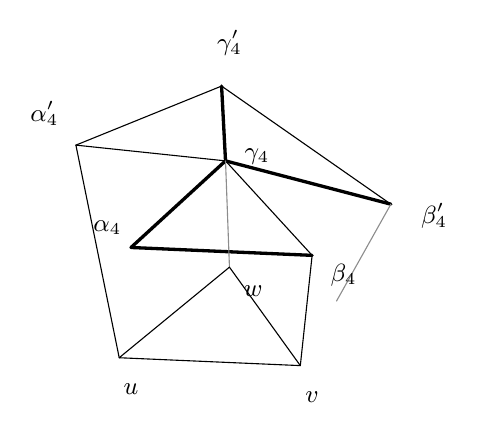
\begin{tikzpicture}[x=1mm,y=1mm,line cap=round,line join=round,font=\scriptsize]
\draw (48.5,-13.5) -- (30,-21);
\draw (48.5,-13.5) -- (70,-28.5);
\draw[very thick] (48.5,-13.5) -- (49,-23);
\draw (30,-21) -- (49,-23);
\draw[very thick] (49,-23) -- (70,-28.5);
\draw[very thick] (37,-34) -- (49,-23);
\draw[very thick] (37,-34) -- (60,-35);
\draw (49,-23) -- (60,-35);
\draw[pencil] (49,-23) -- (49.5,-36.5);
\draw (49.5,-36.5) -- (35.5,-48);
\draw (49.5,-36.5) -- (58.5,-49);
\draw (35.5,-48) -- (58.5,-49);
\draw (30,-21) -- (35.5,-48);
\draw (60,-35) -- (58.5,-49);
\draw[pencil] (70,-28.5) -- (63.1,-40.8);
\node[inner sep=1pt] at (49.5,-8) {\small $\gamma'_4$};
\node[inner sep=1pt] at (26,-17) {\small $\alpha'_4$};
\node[inner sep=1pt] at (75.5,-30) {\small $\beta'_4$};
\node[inner sep=1pt] at (53,-22.5) {\small $\gamma_4$};
\node[inner sep=1pt] at (34,-31.5) {\small $\alpha_4$};
\node[inner sep=1pt] at (64,-37.5) {\small $\beta_4$};
\node[inner sep=1pt] at (52.5,-39.5) {\small $w$};
\node[inner sep=1pt] at (37,-52) {\small $u$};
\node[inner sep=1pt] at (60,-53) {\small $v$};
\end{tikzpicture}
\end{document}
